% !TEX root = ../master.tex
\chapter{Fundamentals}
\label{chap:sota}

TODO forcast on chapter

\section{Computer Vision}

TODO

\ref{fig:sota:imageengineering}
\begin{figure}[hbt]
	\centering
	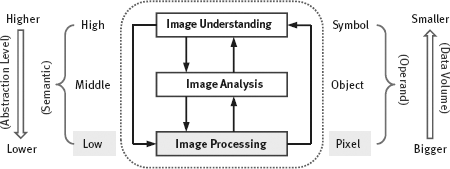
\includegraphics[width=0.8\textwidth, keepaspectratio]{08_Chapter01_fig1-4}
	\caption{\label{fig:sota:imageengineering} Levels of image engineering. 
	Reprinted from \textcite[][Chapter~1]{zhang2017imageprocessing}}
\end{figure}

\subsection{Object Detection}

TODO
edge detection, outline detection
foreground background mask from video image
background substraction

\subsection{Volume Estimation}

TODO
single view, multiview, depth sensors
estimation by pixel area
interpolation of depth information by combinding views
bounding / section box
full 3d reconstruction
\ref{fig:sota:mulitviewtop}

\begin{figure}[hbt]
	\centering
	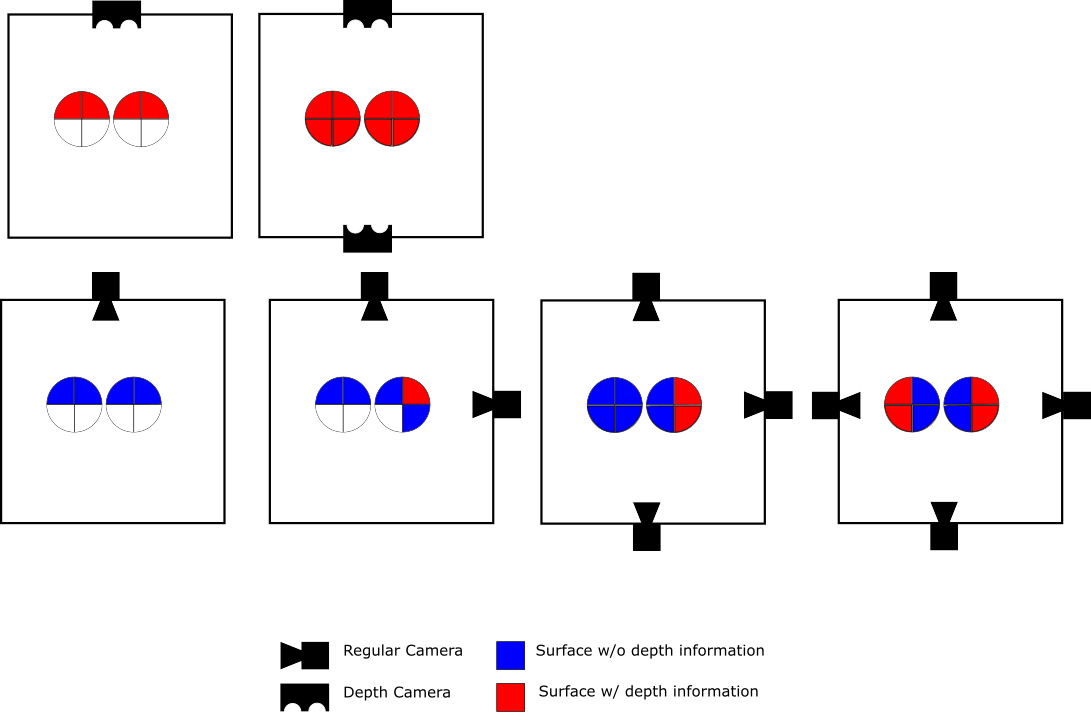
\includegraphics[width=1.0\textwidth, keepaspectratio]{resources/multiview}
	\caption{\label{fig:sota:mulitviewtop}Concept of depth reconstruction in a 2D multi-view situation.
	Based on and adapted from \textcite[][]{sonaten2011volume}}
\end{figure}


\section{Elevator Control}
TODO shor introtuction, definition and what are important aspects about it

\subsection{System Components}

In order to gain an understanding of how an elevator system is controlled,
it is usefull to look at the components a general system uses.


TODO
- shaft and movement mechanism
- motors
- car / cabin / convoyance
- doors
- in cabin panel
- panel on each floor
- advanced cabin sensory
- advanced floor sensory
- door sensors
- control electronic per elevator
-- motor control (cabin dispatch)
-- door control
-- security system
- group controller
TODO find picture or reference

explain call types and typical system behavior

\autocite[][pp.~12-13]{strobl1999controller}
\autocite[][pp.~6,10]{siikonen1997models}
\autocite[][pp.~4,16]{xang2016trafficlist}

\begin{figure}[hbt]
	\centering
	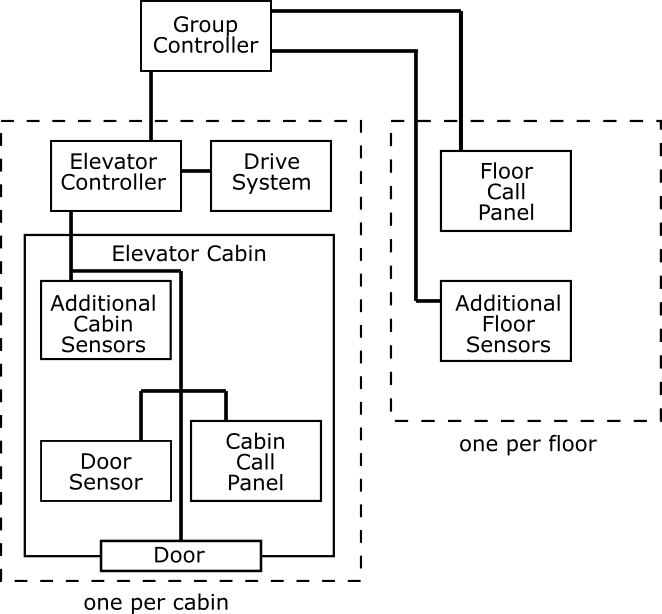
\includegraphics[width=0.8\textwidth, keepaspectratio]{resources/systemcomponets}
	\caption{\label{fig:sota:traffictimes} General components of an elevator control system.}
\end{figure}

\subsection{System Classifications}
TODO
- by amount of elevators
- by type of sensory to haul the car
TODO how many elevators parallel
TODO additional travel information: how many people inside and outside, up / down / floor select inside / outside, everyone presses?, video? 
destination control system
- type of goods / people transported \autocite[][p.~141]{unger2015aufzuege}
-  type of engine / srive system

\subsection{Passenger Traffic Patterns}
Passenger traffic patterns are typical streams of passengers going from one floor to another.
Those patterns are reoccurring regularly based on the time of the day.
The movement of passengers can be described with three directions: \emph{incoming}, \emph{outgoing}, and \emph{inter-floor} traffic.
With those directions the traffic patterns can be described, as they focus on one of the directions, but also incorporates components of passengers heading in other directions \autocite[][p.~259]{siikonen1993simulation}.
According to multiple sources, three general patterns are present in office buildings \autocite[][pp.~1--2]{beers2015arrivals}
\autocite[][pp.~6--7]{axelsson2013strategies}
\autocite[][p.~194]{unger2015aufzuege}
\autocite[][p.~14]{siikonen1997models}:

\begin{itemize}
    \item \textbf{Up-peak traffic} In the morning the majority of passengers in an office building constitutes to an incoming traffic.
    They arrive at the entrance lobby and travel to different upper floors to fill the building.
    The lift cars potentially need to stop at every level and return to the lobby without passengers to pick up new ones. 
    This reduces the utilized capacity and puts a high load on the elevator system to convoy all passengers in time.
    \item \textbf{Down-peak traffic} In the evening the majority of the passengers are leaving the office building and travel from arbitrary upper floors to the main lobby.
    Most of the passengers constitute to outgoing traffic.
    The elevator system needs to pick up passengers at every level. 
    Reverse to the up-peak traffic, the cars are empty when returning from the lobby.
    Similar to the up-peak traffic this situation induces a high stress on the system.
    \item \textbf{Inter-floor traffic} All other traffic that is neither incoming nor outgoing can be considered inter-floor traffic. Passengers that travel from one floor to another but are not entering or leaving the building are the majority in this situation.
\end{itemize}

%Figure \ref{fig:sota:trafficpatterns} depicts the former mentioned traffic components.
Figure \ref{fig:sota:traffictimes} shows an example of how the traffic components contribute to overall traffic in an office building. A clear peak of incoming traffic in the morning and outgoing traffic in the evening are visible.
This information can be used to model simulations and predict traffic in various circumstances.
It has significant impact on the scheduling principles employed for each situation in order to improve the efficiency of an elevator system.

%\begin{figure}[hbt]
%	\centering
%	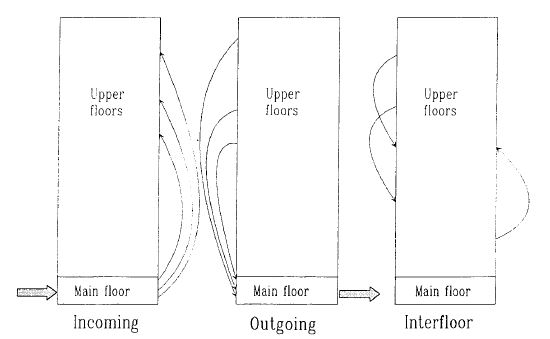
\includegraphics[width=0.8\textwidth, keepaspectratio]{resources/trafficpatterns}
%	\caption[]{\label{fig:sota:trafficpatterns} Typical categories of passenger traffic: Incoming, Outgoing and Inter-floor.
%	Reprinted from \textcite[][p.~259]{siikonen1993simulation}}
%\end{figure}

\begin{figure}[hbt]
	\centering
	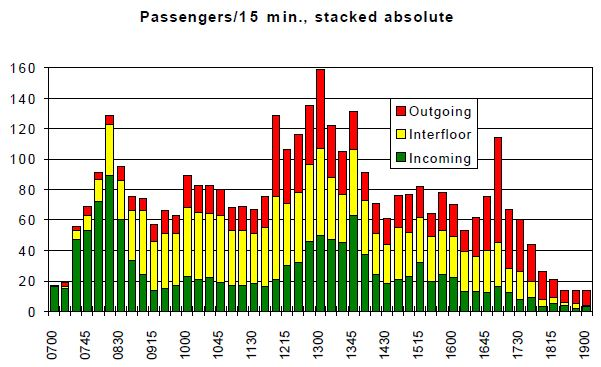
\includegraphics[width=0.8\textwidth, keepaspectratio]{resources/traffictimes}
	\caption{\label{fig:sota:traffictimes} Exemplary traffic component profile for an office building.
	Reprinted from \textcite[][p.~14]{siikonen1997models}}
\end{figure}

TODO layout the figures
TODO or use \textcite[][p.~12]{sorsa2005destination} as broader image 

\subsection{Control Strategies}
TODO

\autocite[][pp.~3--4,10]{beers2015arrivals}
- stopping policies / strategies
- parking polcies
- call allocation

\autocite[][pp.~3--6]{axelsson2013strategies}
- collective control
- zoneing
- search based
- rule based
- genetic algorithm




\subsection{Performance Criteria}

In order to evaluate the performance of an elevator system some metrics about it are commonly considered.
They are used to check if a planned system fulfills the requirements that the expected traffic poses. 
The metrics are mostly perceived as part of the service quality by the passengers.
Many of them are linked together and influence each other.

% General cite:
%\autocite[][p.~10]{beers2015arrivals}
%\autocite[][p.~7]{hakonen2003simulation}
%\autocite[][pp.8-9]{siikonen1997models}
%\autocite[][p.~194]{unger2015aufzuege}

\begin{itemize}

    \item The \textbf{passenger waiting time} 
        describes the amount of time between the arrival of a passenger at the landing floor 
        and their entry into the elevator cabin. 
        \autocite[][p.~7]{hakonen2003simulation}\autocite[][pp.8-9]{siikonen1997models}
        
    \item The \textbf{passenger ride time} 
        measures the time between the entering of a passenger into the cabin 
        and them exiting the cabin on the destination floor. 
    \autocite[][pp.8-9]{siikonen1997models}
    
    \item The \textbf{total journey time}, 
        also called \emph{total service time} \autocite[][p.~10]{beers2015arrivals} or \emph{time to destination},
        describes the total time a passenger spends in the system 
        and is calculated by the sum of waiting and ride time.
        \autocite[][pp.8-9]{siikonen1997models}
        
    \item The \textbf{round trip time} 
        describes the time it takes for a single elevator to collect passengers at the lobby,
        deliver them to the upper floors and return to the lobby. 
        This measure is critical in the up-peak traffic.
        \autocite[][pp.8-9]{siikonen1997models}
        
    \item The \textbf{handling capacity}, 
        also called \emph{5-minute interval}
        \autocite[][p.~194]{unger2015aufzuege},
        describes the maximum number of passengers that can be transported (into the upper most floor) during up-peak traffic.
        \autocite[][pp.8-9]{siikonen1997models}
        It is dependent on the round trip time.
        In theoretical considerations a maximum utilization of 60-80\% of the capacity is used for this scenario. 
        \autocite[][p.~194]{unger2015aufzuege}\autocite[][p.~7]{hakonen2003simulation}
    
    \item The \textbf{interval time} 
        describes the time between departures of any cabin from the lobby 
        and influences the time a passenger hat to wait at the lobby.
        \autocite[][pp.8-9]{siikonen1997models}
    
    \item The \textbf{hall call time} 
        describes the time between the issuing of an hall call by a passenger and the cancellation of the call. 
        The call is canceled when an elevator is scheduled to serve the call floor and hence decelerates to stop at the floor.
        \autocite[][pp.8-9]{siikonen1997models} 
    
    \item The number of \textbf{total stops}
        necessary to serve an specified amount of passengers (or within a given time frame) is an indicator for the efficiency of the scheduling algorithm.
        \autocite[][p.~194]{unger2015aufzuege}
    
    \item The \textbf{energy consumption} 
        per ride or per time interval is an measure of economic interest. 
        However it does not influence the perceived service quality.
    
    \item The \textbf{capacity utilization} 
        of the cabins in spacial and weight dimensions is an interesting metric to observe, 
        since usually only 60-80\% of the capacity is used at a time. 
        \autocite[][p.~194]{unger2015aufzuege}
        \autocite[][p.~7]{hakonen2003simulation} 
        This utilization can be even lower when large objects are present.
        The average utilization is further influenced by empty rides.
        
\end{itemize}

For each of the metrics it is common to calculate statistical figures, such as average, mean, minimum, maximum and standard deviation, which also can differ depending on the traffic situation.
These calculations can be based on theoretical consideration about the physical parameters of the system \autocite[][p.~194]{unger2015aufzuege}, simulations or heuristical observations in real buildings.
 



\subsection{Simulational Optimization Approaches}
TODO
model building etc: here is a lot of research in the topic utilizing theoretical multivariable model optimization, simulational approaches and heuristical approaches in real world (refs?)

\autocite[][pp.~7--11]{beers2015arrivals}
\autocite[][p.~193]{unger2015aufzuege}


TODO
